\section*{Memory Management}
\subsection*{Main Memory}
MM is the only storage the CPU can access directly. \textbf{Speed:} CPU Registers > Cache > Main Memory.
% Main Memory Partitions: resident OS in high PA, user processes usually in low pa
    \textbf{Base and limit registers} smallest legal mem. address + size. Define \textbf{Logical Address Space (LAS)} of a P (set of all LA's). P can only access memory inside LAS (otherwise trap $\rightarrow$ fatal error). Only OS can access all registers/memory. \\
    \textbf{Logical Address / Virtual Address} generated by CPU. visible to user. editable \\
    \textbf{Physical Address} only seen by Memory Unit. does not change. \textbf{PAS} set of  all PAs correspoding to LAS \\
    \textbf{Address Binding} mapping instructions and data to memory addresses. 3 schemes/stages: (in red) \\
    \begin{wrapfigure}{r}{0.15\linewidth}
        \vspace{-12pt}
        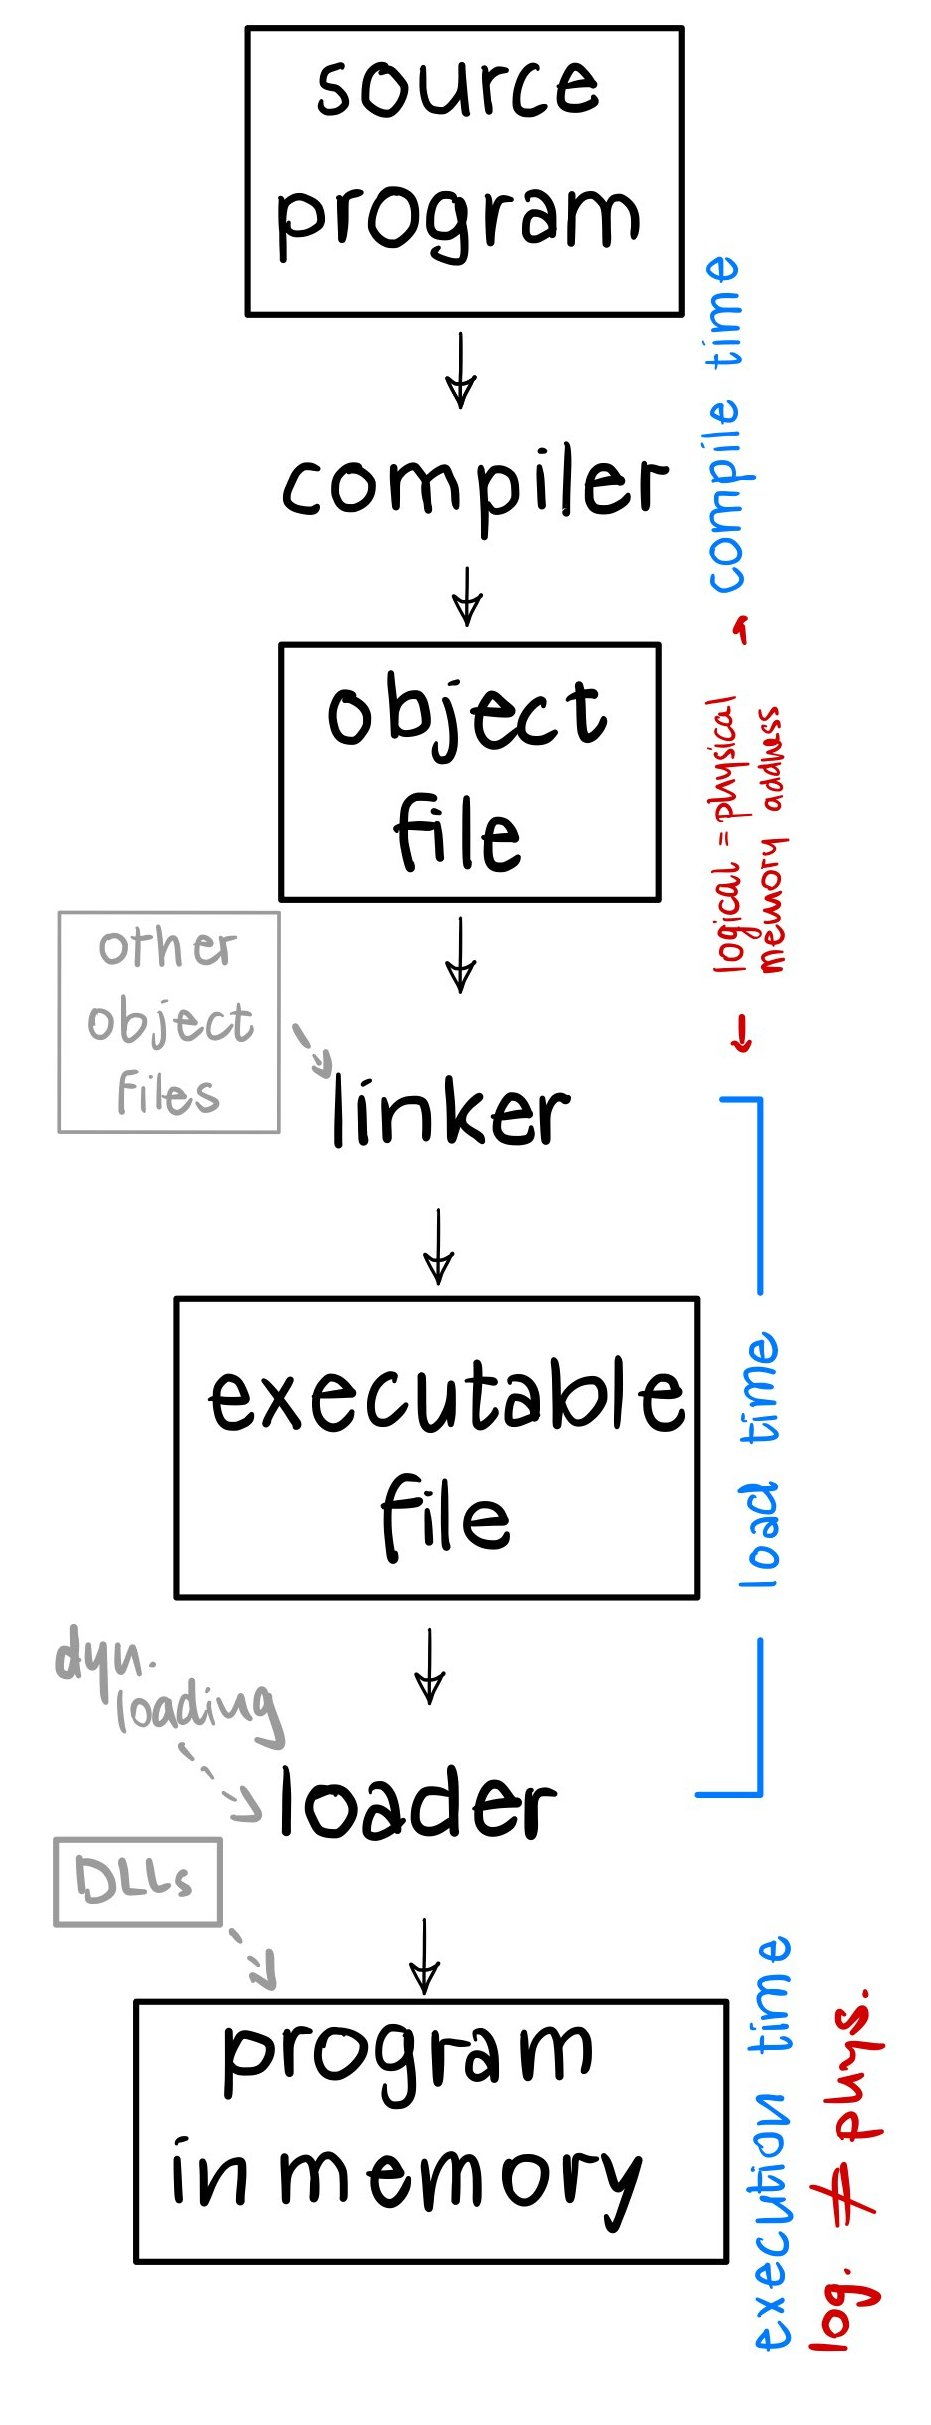
\includegraphics[width=\linewidth]{05_mem.jpg}
        \vspace{-60pt}
    \end{wrapfigure}
    \textbf{Memory Management Unit MMU} HW device, maps LA to PA during execution. $\rightarrow$ mapping methods (relocation register, contiguous paging) \\
    \textbf{Dynamic Loading}: routine not loaded in memory until called. all routines kept on disk. no special os support needed \textbf{Static Linking}: Libraries and program code combined by loader. \textbf{Dynamic Linking} happens during execution. useful for shared libraries (standard C lib.) DLL: dynamically linked libraries. \\
    \textbf{Contiguous Memory Allocation} each process is contained in a single section of memory that is contiguous to the section containing the next process. \textbf{Memory Protection:} through usage of Relocation \& limit registers. degree of multiprog. limited by nr of partitions. \\
    \textbf{Dynamic Storage Allocation}: OS maintains list of allocated and free partitions (\textbf{Holes}). First-fit (fastest), Best-fit (eq. to ff in storage-utilization, produces smallest leftover-hole), worst-fit (produces largest leftover hole) \\
    \textbf{Internal Fragmentation }: physical memory organized into fixed-size blocks. happens if allocated memory larger than requested memory (internal to partition). \\
    \textbf{External Fragmentation }: Total Memory Space for requests exists, but is not contiguous. 50\% rule: 1/3 unusable. \textbf{Solutions} \textit{Compaction}: moving data, can be expensive, only possible with dynamic address relocation (during ex. time) \textit{Noncontinguous Allocation}: Strategy used in Paging \\
    \textbf{Paging } PA can be noncontiguous, memory for P allocated wherever possible (no ex. fragmentation, but some internal $\rightarrow$ smaller pages eq. less int. frag but move overhead in page table). Physical memory is divided into fixed-size blocks called \textbf{frames}. Logical memory divided into same-sized blocks called \textbf{pages}.\\
        \begin{itemize}
            \item \textbf{Adress-Translation}: page number and page offset in the per-process page table
                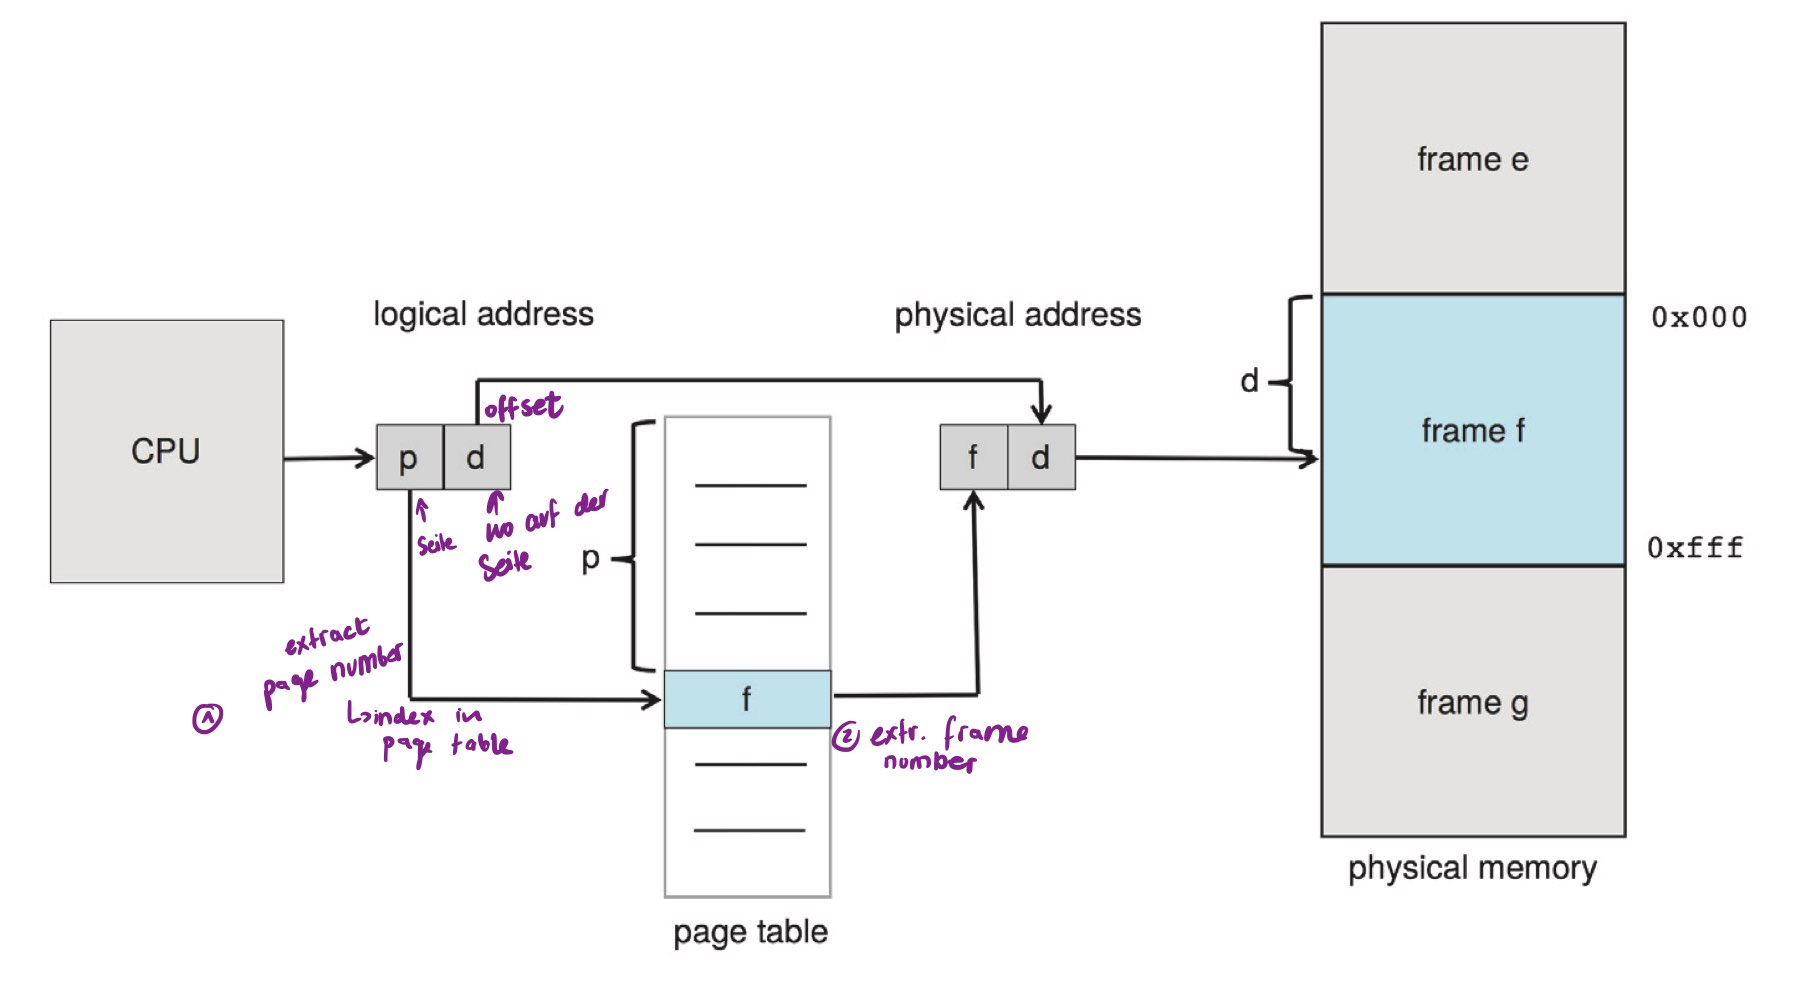
\includegraphics[width=0.5\linewidth]{05_paging.jpg} %TODO: modify image to include TLB
            \item OS keeps copy of each per-process page table + maintains frame table (for each physical frame)
            \item \textbf{Hardware Implementation}: per-process page table kept in main memory. \textbf{PTBR} page-table base register (pointers) \& \textbf{PTLR} page-table length register (size of page table)
            \item \textbf{Translation Lookaside Buffer TLB}: also called associative memory. hw cache for page table. (page nr, frame)
                % replacement policies: round-robin, LRU, random. key kernel code can be wired down for permanent fast access
            \item \textbf{Memory Protection} protection bit (read-only, read-write) or valid-invalid bit (attached to each entry in the page table. indicates if legal (in LAS) or not)
            \item \textbf{Shared Pages}: reentrant (unchanging) code shared among processes. ex: Standard C libary
        \end{itemize}
        \textbf{Structure of the Page Table} \\
        \textbf{Hierarchical Page Table}: ex: two-level page table, page the page table. (forward mapping) \\
        \textbf{Swapping}: moving process temporarily out of memory to a \textit{backing store} and brought back for continued execution. (process roll out, roll in). system maintains ready queue. $\rightarrow$ transfer time too high, not used in modern OS  \\
%TODO: hashed page tables, inverted page tables (if addresses expand beyond 32bits)
        \textbf{Swapping with Paging}: pages of a process instead of whole process swapped. (page in, page out)
\subsection*{Virtual Memory}
Abstracts main memory into an extremely large, uniform array of storage (LAS > PAS). Allows execution of partially-loaded programs. (more programs can run at the same time, increased CPU utilization \& throughput, no increase in reponse/turnaround time, less I/O needed to swap processes )
\begin{description}
    \item[Demand Paging]
    \item[Copy-on-Write]
    \item[Page Replacement]
    \item[Allocation of Frames]
    \item[Thrashing]
    \item[OS Examples]
\end{description}
